\documentclass{article}
\usepackage[margin=1in]{geometry}
\usepackage[pdftex]{graphicx}
\usepackage{cite}
\usepackage{color}
\usepackage{listings}
\usepackage{pdfpages}
\definecolor{mygreen}{rgb}{0,0.6,0}
\definecolor{mygray}{rgb}{0.9,0.9,0.9}
\definecolor{mymauve}{rgb}{0.58,0,0.52}
\lstset{
  backgroundcolor=\color{mygray},     % choose the background color; you must add \usepackage{color} or \usepackage{xcolor}
  basicstyle=\tiny\ttfamily,  % the size of the fonts that are used for the code
  breakatwhitespace=false,            % sets if automatic breaks should only happen at whitespace
  breaklines=true,                    % sets automatic line breaking
  captionpos=b,                       % sets the caption-position to bottom
  commentstyle=\color{mygreen},       % comment style
  deletekeywords={...},               % if you want to delete keywords from the given language
  escapeinside={\%*}{*)},             % if you want to add LaTeX within your code
  extendedchars=true,                 % lets you use non-ASCII characters; for 8-bits encodings only, does not work with UTF-8
  frame=single,                       % adds a frame around the code
  keepspaces=true,                    % keeps spaces in text, useful for keeping indentation of code (possibly needs columns=flexible)
  keywordstyle=\color{blue},          % keyword style
  language=Verilog,                   % the language of the code
  morekeywords={*,...},               % if you want to add more keywords to the set
  numbers=left,                       % where to put the line-numbers; possible values are (none, left, right)
  numbersep=5pt,                      % how far the line-numbers are from the code
  numberstyle=\tiny\color{mygray},    % the style that is used for the line-numbers
  rulecolor=\color{black},            % if not set, the frame-color may be changed on line-breaks within not-black text (e.g. comments (green here))
  showspaces=false,                   % show spaces everywhere adding particular underscores; it overrides 'showstringspaces'
  showstringspaces=false,             % underline spaces within strings only
  showtabs=false,                     % show tabs within strings adding particular underscores
  stepnumber=2,                       % the step between two line-numbers. If it's 1, each line will be numbered
  stringstyle=\color{mymauve},        % string literal style
  tabsize=1,                          % sets default tabsize to 2 spaces
  %title=\lstname                      % show the filename of files included with \lstinputlisting; also try caption instead of title
}
\title{EEE 178: Homework 2}
\date{\today}
\author{Curtis Muntz}
\begin{document}
\maketitle
\begin{itemize}
	\item Problem 2
	\begin{itemize}
		\item Part 10
		\item[] As you can see in the images attached on the following pages, the gaussian filter was slightly effective in removing the gaussian noise, and the median filter was very effective in removing the salt \& pepper noise. Both filters were very ineffective at removing the other form of noise. See Table \ref{table:filtertable}
		\item[] All of the functions that I wrote were effective in producing identical results as the built in functions, but ran exponentially slower than their counterparts.
		\item[] See the attached pages for the MATLAB code used to complete the homework and self-written functions. 


	\end{itemize}
\end{itemize}

\begin{table}[ht]
\caption{Filter Effectiveness On Noise Type}
\centering
\begin{tabular}{c c c}
\hline
\hline
Filter Type & Noise Type & Results\\
\hline
Gaussian & Gaussian Noise & Sort of effective\\
Median & Salt \& Pepper Noise & Very effective\\
Gaussian & Salt \& Pepper Noise & Not effective\\
Median & Gaussian Noise & Not effective \\
\hline
\end{tabular}
\label{table:filtertable}
\end{table}

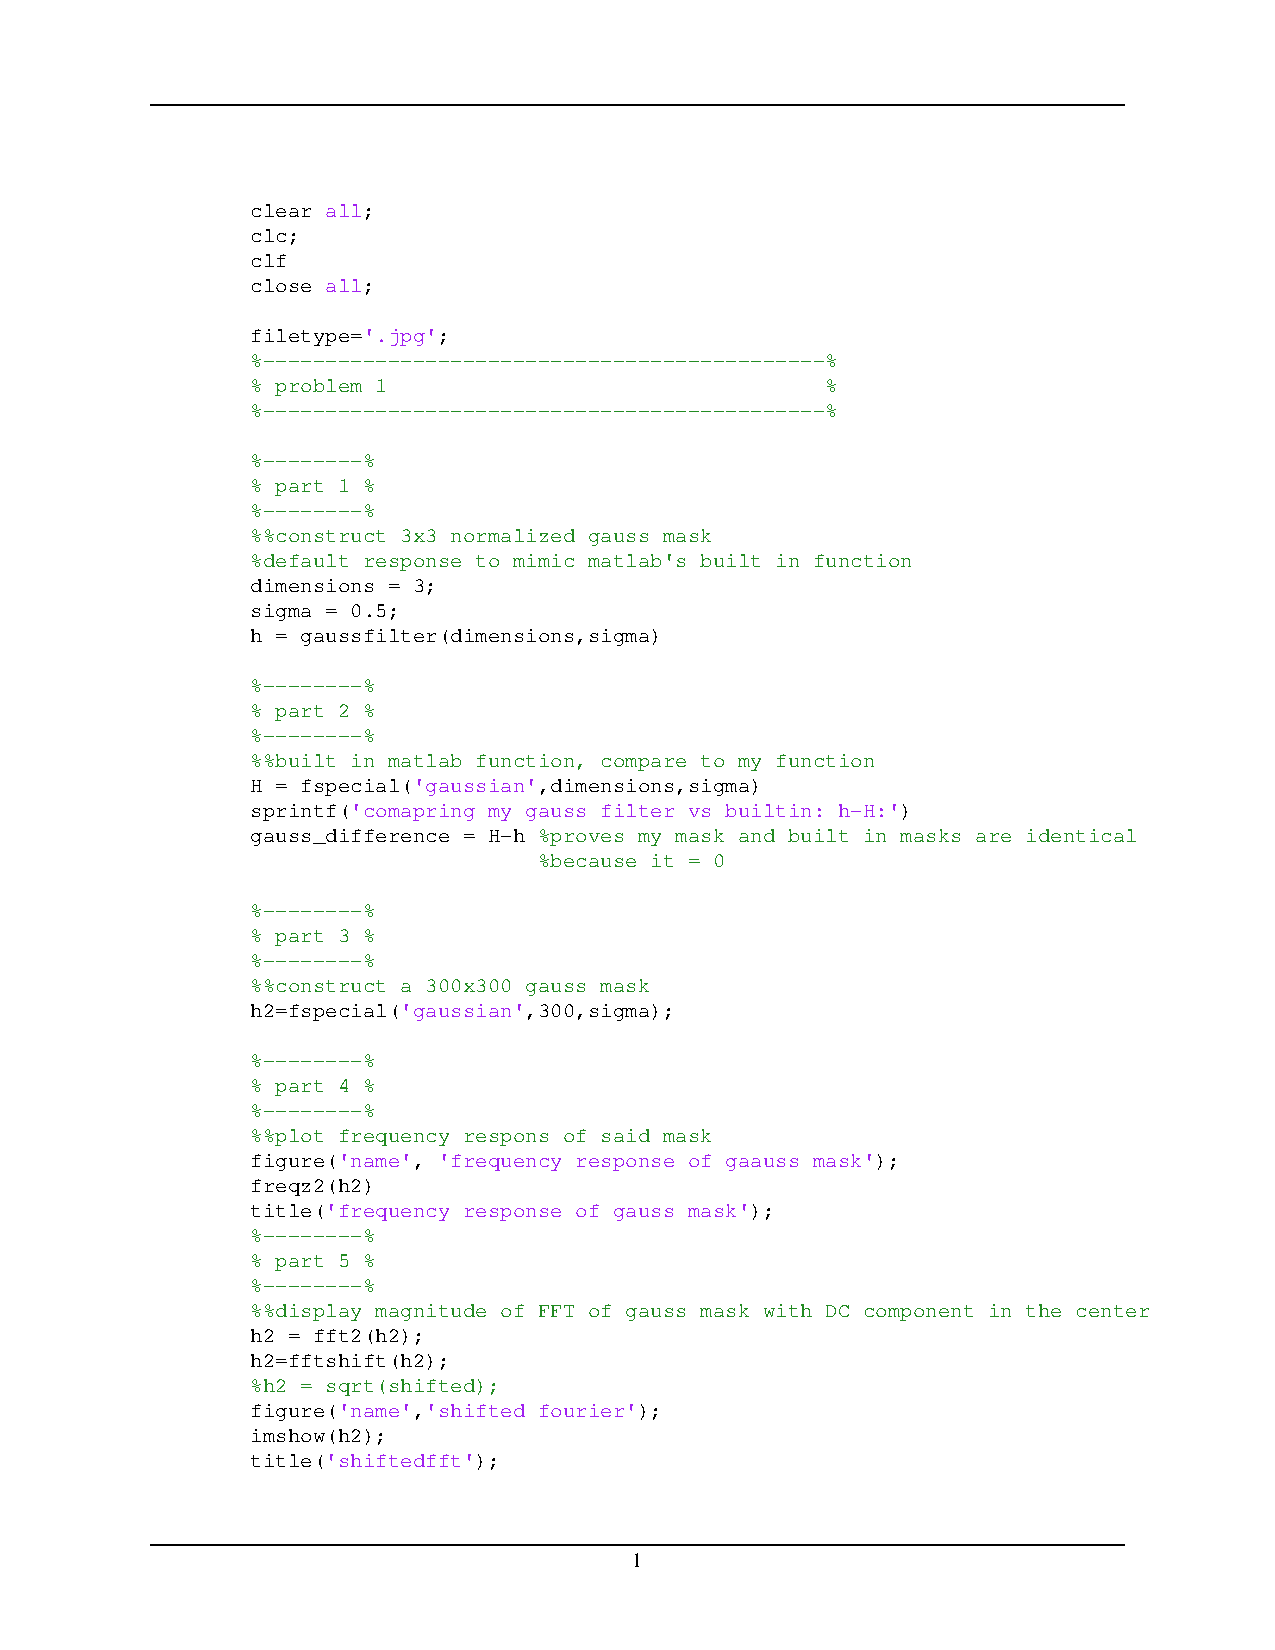
\includepdf[pages={1-12}]{../html/hw2.pdf}
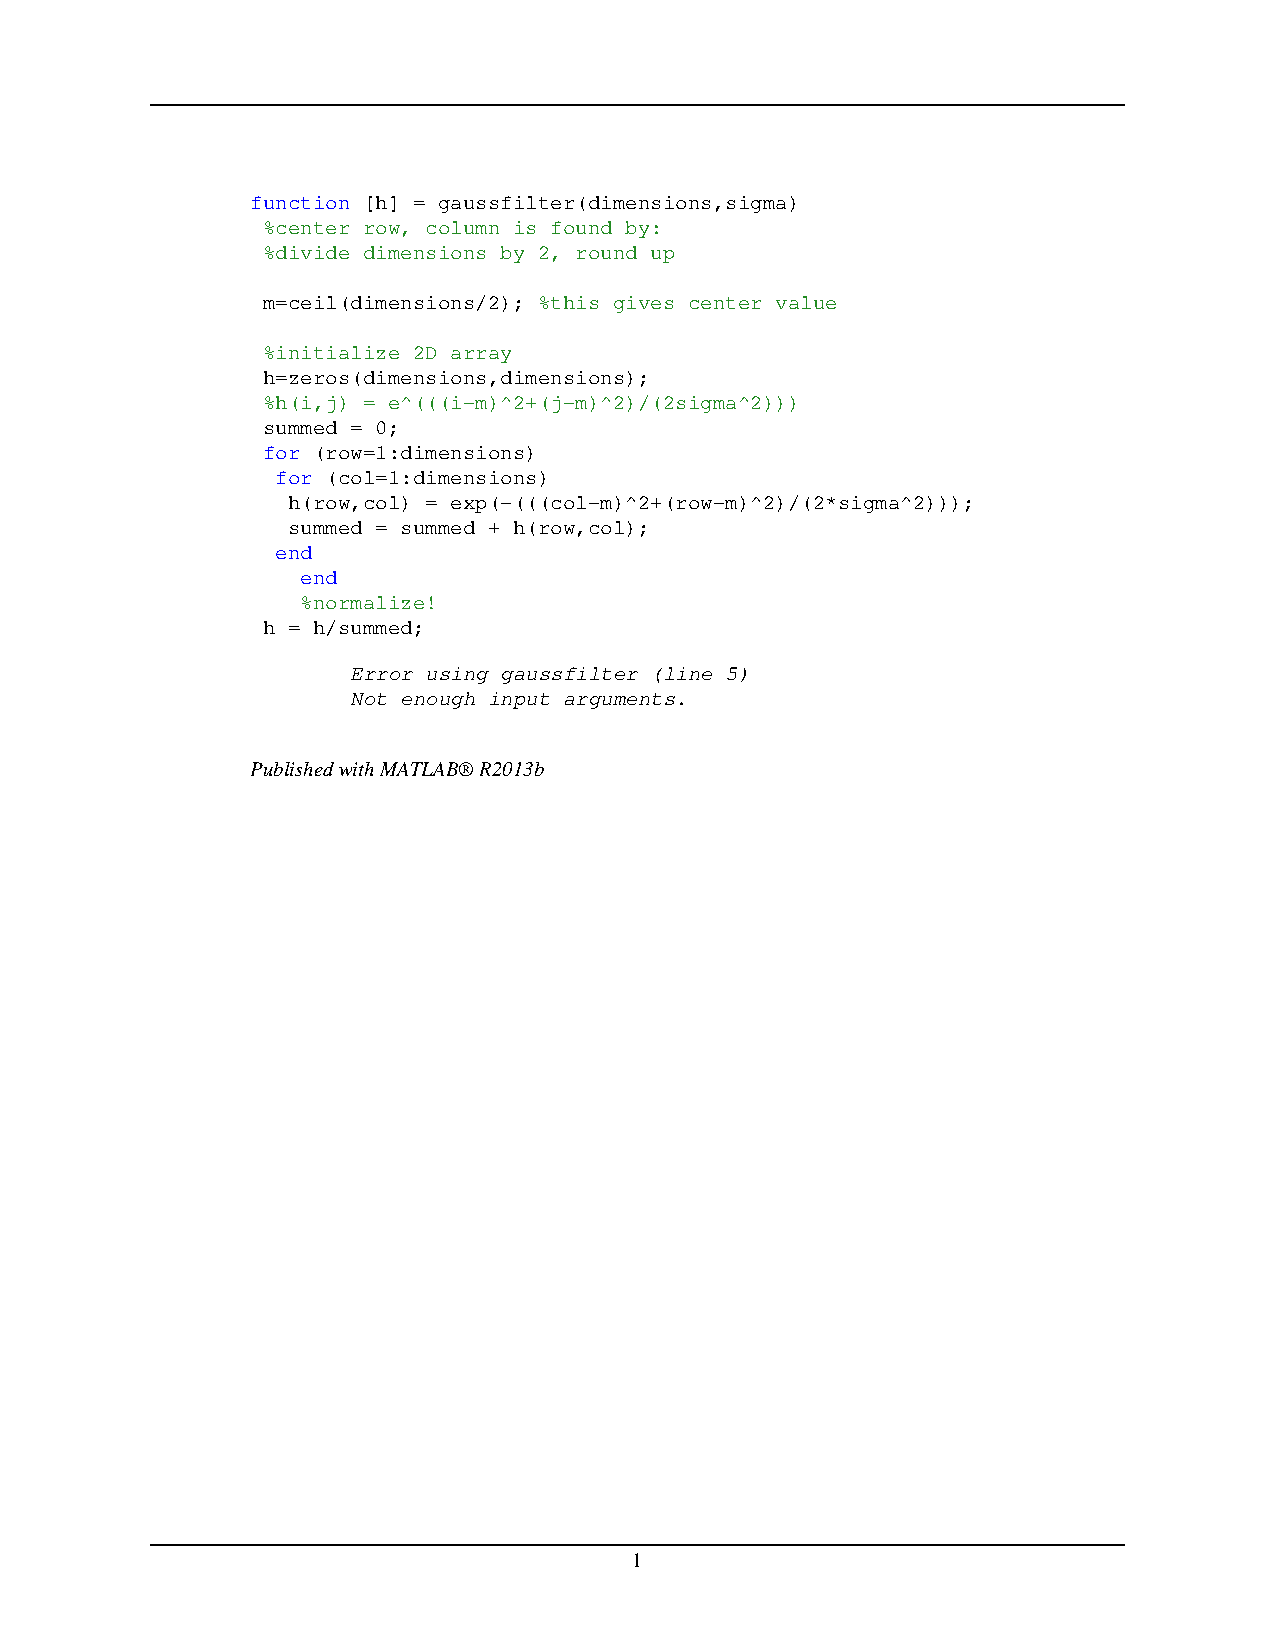
\includepdf[pages={1}]{../html/gaussfilter.pdf}
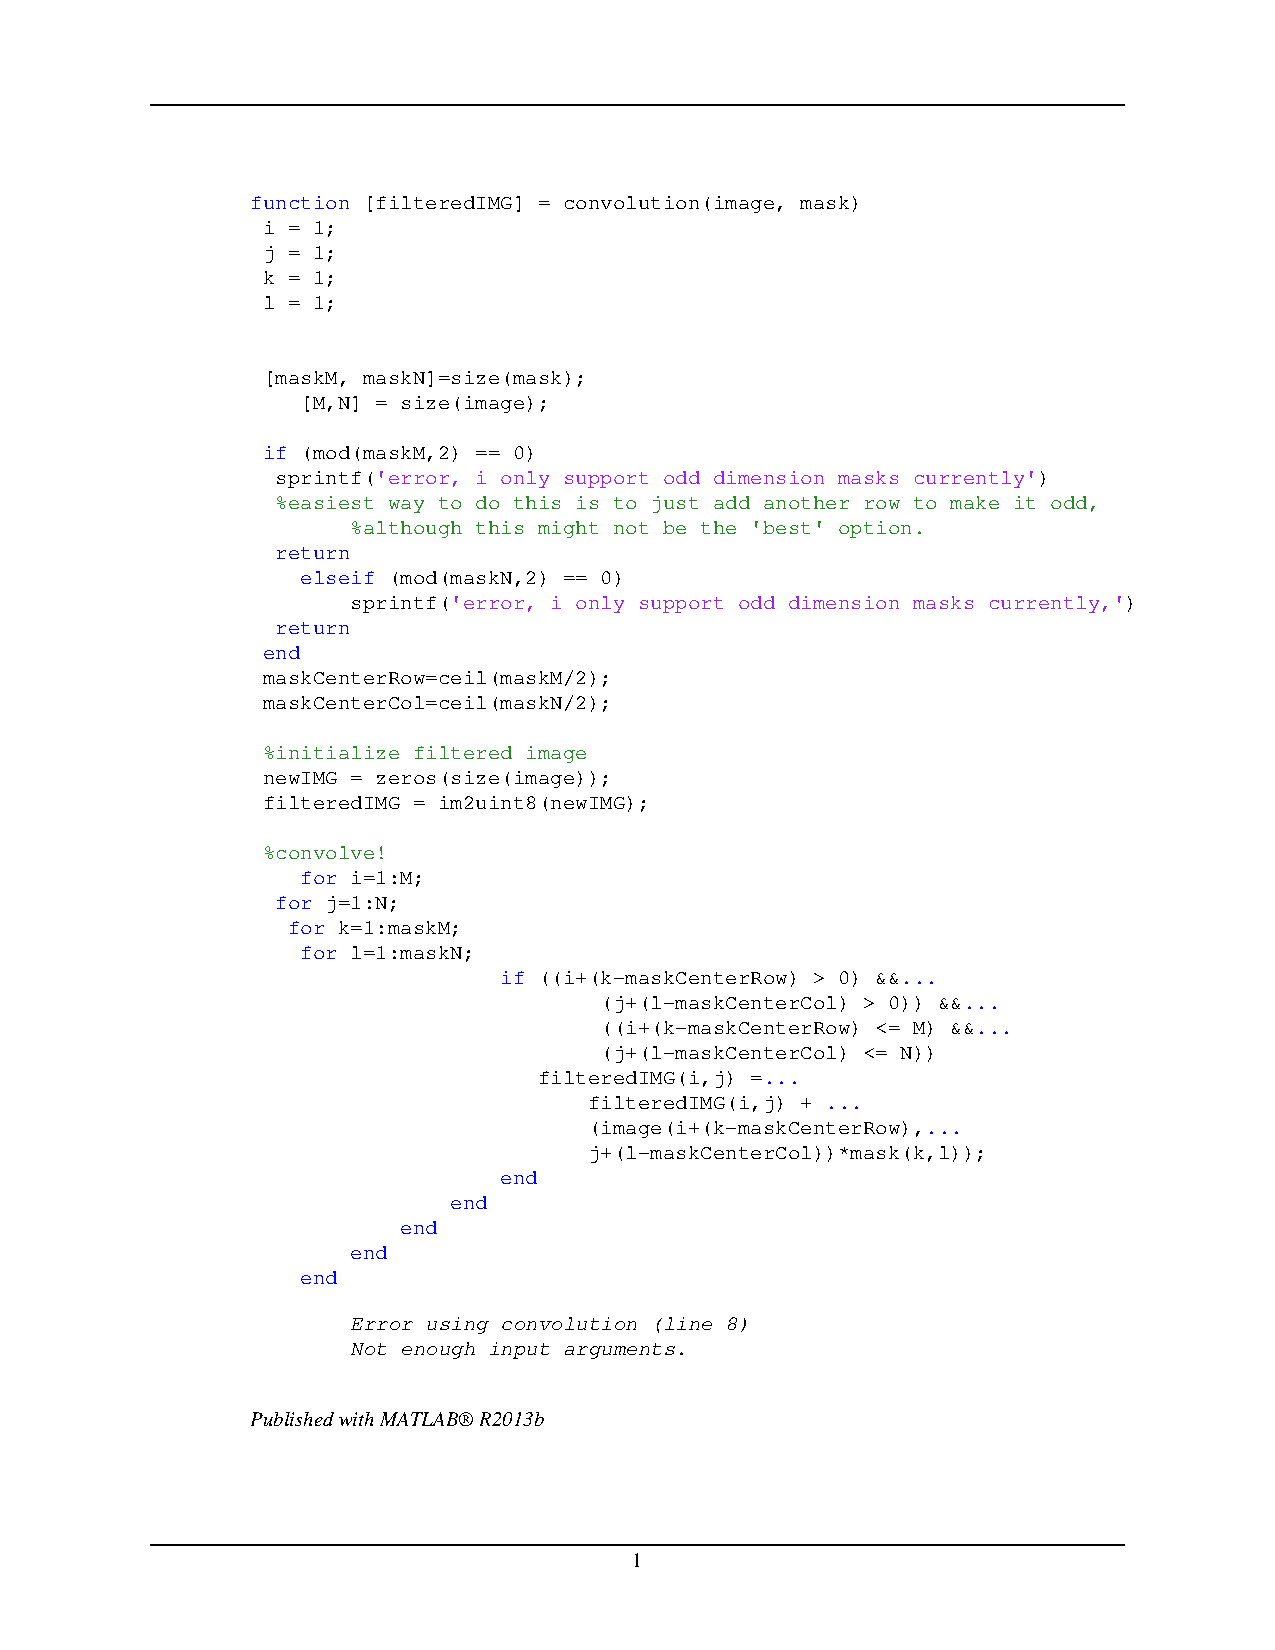
\includepdf[pages={1}]{../html/convolution.pdf}
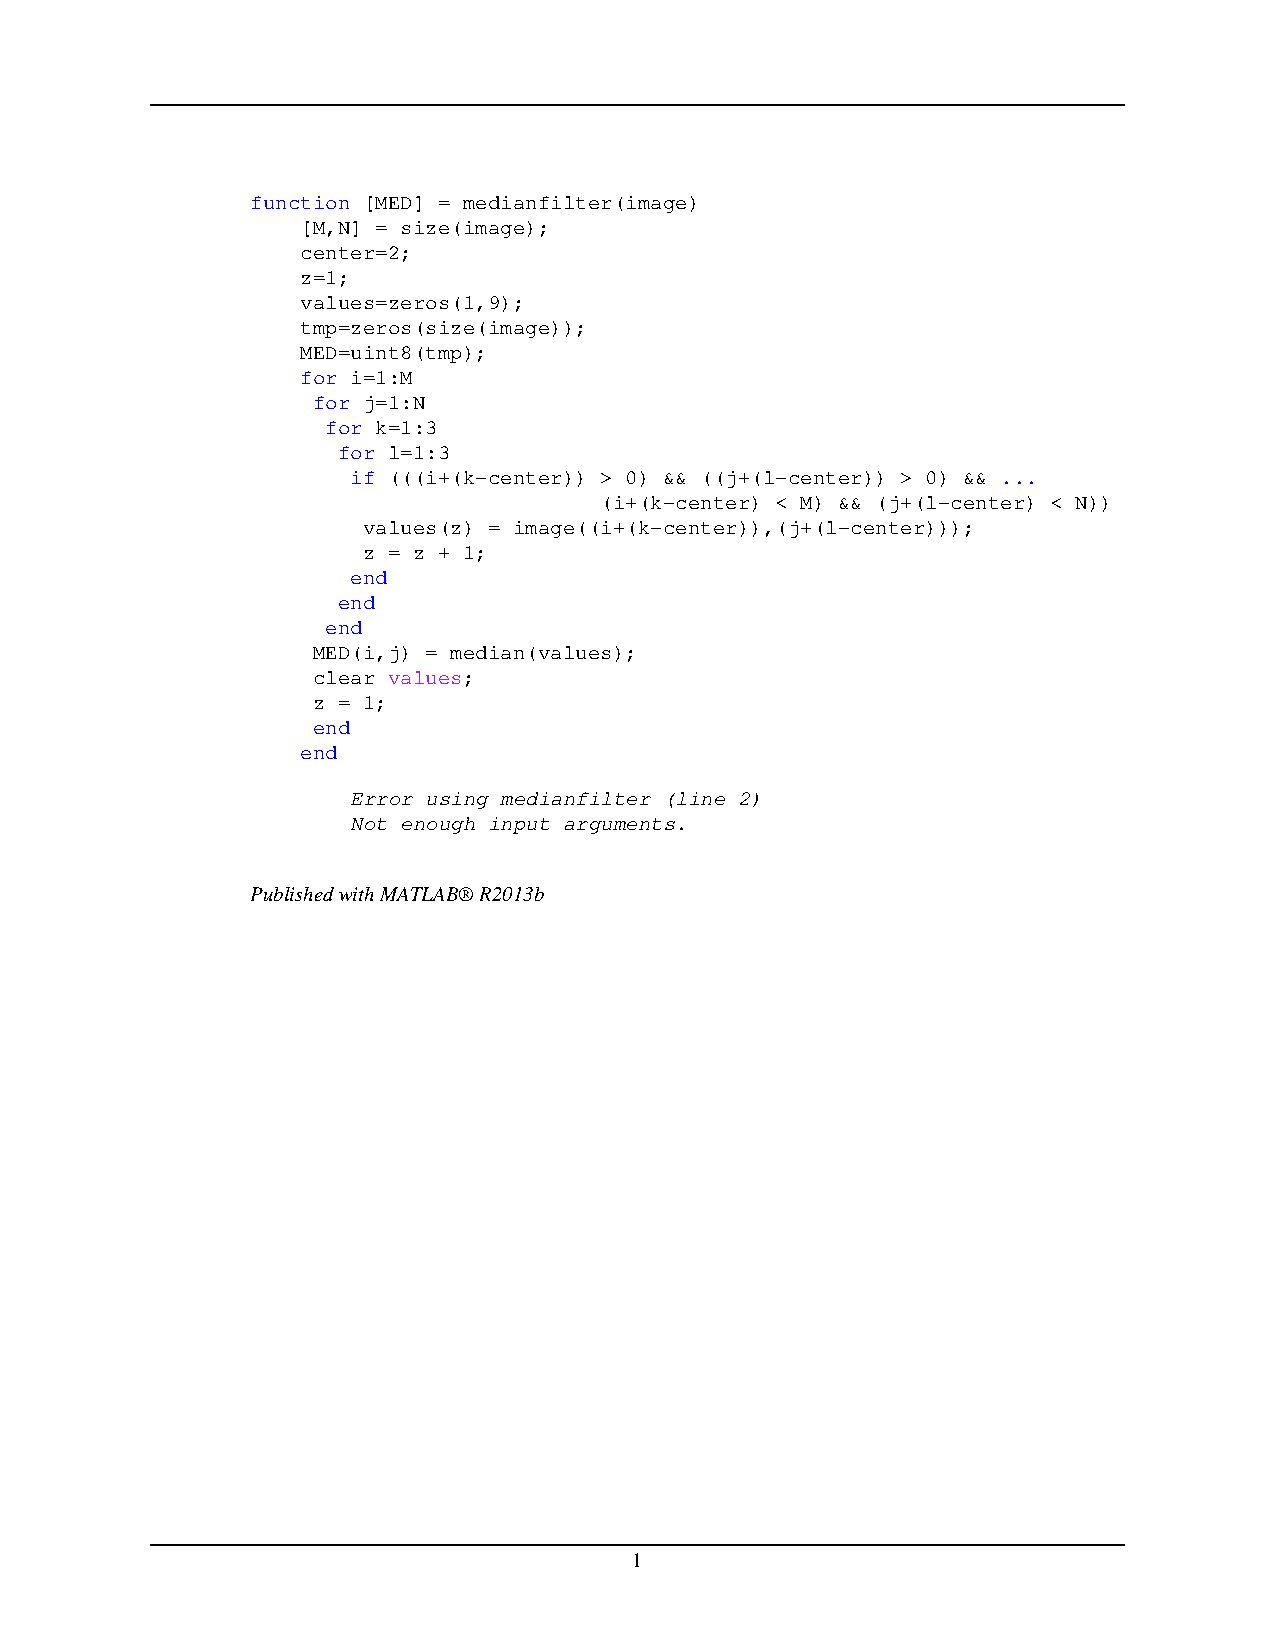
\includepdf[pages={1}]{../html/medianfilter.pdf}
\end{document}